\section{Symmetry and energy-conservation checks}

This section collects three stress tests that do not rely on a closed-form
comparison curve but on exact symmetries and conservation laws of the
underlying electromagnetic problem. Any departure from these identities
points to a structural bug rather than a tabulation error.

The first test checks Lorentz reciprocity of the intensity transmittance.
An asymmetric four-layer absorbing stack with refractive indices
$(n_0, n_1, n_2, n_3, n_s) = (1.00,\ 1.50+0.02\,\ii,\ 2.50+0.10\,\ii,\
3.50+0.05\,\ii,\ 1.80)$ and thicknesses
$(d_1, d_2, d_3) = (\SI{120}{}, \SI{80}{}, \SI{50}{\nano\metre})$ is
evaluated at normal incidence across
$\lambda \in [\SIrange{400}{1000}{\nano\metre}]$, and then the whole stack
is reversed. The amplitude transmittance $t$ is not reciprocal in general,
but the intensity transmittance $T$ is, for any linear, time-reversal-even
medium:
\begin{equation}
  T(\mathrm{fwd}) = T(\mathrm{rev}). \label{eq:sym-rec}
\end{equation}
Reciprocity holds even when the interior of the stack is absorbing, which
is why the test materials above carry non-zero $\Imy(n_j)$; the only
restriction is that the bounding half-spaces are lossless, which is the
case ($\Imy(n_0) = \Imy(n_s) = 0$).

The second test checks the sign convention at normal incidence. For any
stack (lossy or lossless, isotropic, non-magnetic), $r_s$ and $r_p$ must
coincide at $\theta_0 = 0$ because the two polarisations are physically
indistinguishable there. The code uses the convention that enforces this
identity without a sign flip, and the test verifies it on 20 randomly
generated stacks with $L \in [1, 4]$ layers, complex indices
$n_j = (1 + U_j) + \ii\,U'_j$ with $U_j \sim \mathcal{U}(0, 3)$ and
$U'_j \sim \mathcal{U}(0, 0.2)$, thicknesses
$d_j \sim \mathcal{U}(\SI{20}{}, \SI{300}{\nano\metre})$, at
$\lambda = \SI{600}{\nano\metre}$:
\begin{equation}
  r_s(\theta_0 = 0) = r_p(\theta_0 = 0). \label{eq:sym-normal}
\end{equation}

The third test checks energy conservation for a lossless DBR under an
angular sweep. The stack is five quarter-wave pairs of
TiO$_2$ ($n_H = 2.35$) / SiO$_2$ ($n_L = 1.46$) on a transparent substrate
($n_s = 1.5$) at $\lambda_0 = \SI{550}{\nano\metre}$, evaluated for
$\theta_0 \in [0, \SI{85}{\degree}]$ in both polarisations. Because all
materials are real,
\begin{equation}
  R + T = 1. \label{eq:sym-energy}
\end{equation}

\begin{center}
\begin{tikzpicture}
  \fill[black!4]   (0, 0) rectangle (5, 1.2);
  \fill[red!10]    (0,-0.4) rectangle (5, 0);
  \fill[red!20]    (0,-0.8) rectangle (5,-0.4);
  \fill[red!30]    (0,-1.2) rectangle (5,-0.8);
  \fill[blue!6]    (0,-1.9) rectangle (5,-1.2);
  \draw[thick] (0,0) -- (5,0);
  \draw[thick] (0,-1.2) -- (5,-1.2);
  \node[lbl, anchor=east] at (4.9, 0.9) {$n_0$};
  \node[lbl, anchor=east] at (4.9,-0.2) {$n_1$};
  \node[lbl, anchor=east] at (4.9,-0.6) {$n_2$};
  \node[lbl, anchor=east] at (4.9,-1.0) {$n_3$};
  \node[lbl, anchor=east] at (4.9,-1.55){$n_s$};
  \draw[-{Latex[length=1.5mm]}, thick, gray] (0.3,-2.3) -- (4.7,-2.3);
  \node[lbl, gray] at (2.5,-2.55) {reverse};
  \raysketch{1.6}{30}{f}
\end{tikzpicture}
\end{center}

\begin{figure}[!htbp]
  \centering
  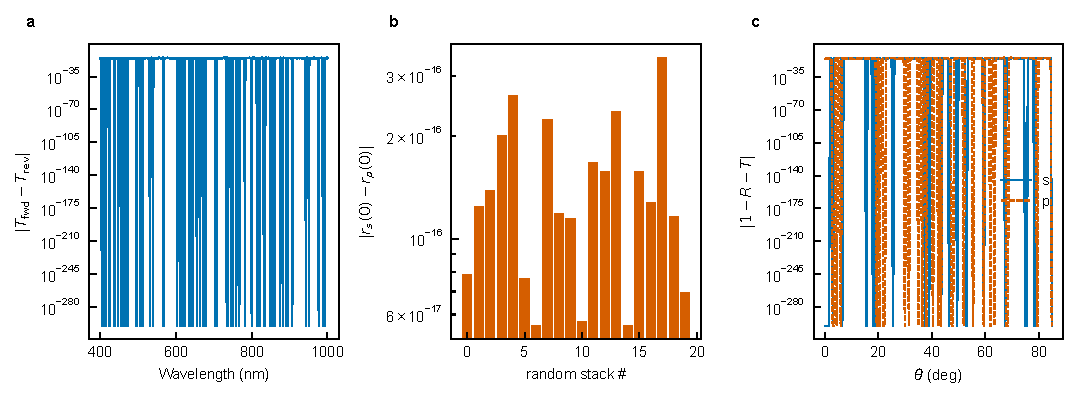
\includegraphics[width=\textwidth]{13_symmetry_checks.pdf}
  \caption{(a) Lorentz reciprocity $|T_{\rm fwd} - T_{\rm rev}|$ against wavelength for the absorbing asymmetric stack. (b) $|r_s - r_p|$ at normal incidence over 20 random stacks. (c) Energy-conservation residual $|1 - (R + T)|$ for a lossless five-pair DBR as a function of angle, in both polarisations.}
  \label{fig:sym}
\end{figure}

Reciprocity holds at
$\max|T_{\rm fwd} - T_{\rm rev}| \approx \num{2e-15}$, the normal-incidence
identity at $\max|r_s(\theta_0 = 0) - r_p(\theta_0 = 0)| \approx
\num{3e-16}$ over the 20 random stacks, and energy conservation of the
lossless DBR at $\max|1 - (R + T)| \approx \num{4e-15}$ over the full
angular sweep. The three residuals probe independent parts of the
formalism: \eqref{eq:sym-rec} exercises the stack-reversal algebra of the
transfer matrix, \eqref{eq:sym-normal} exercises the Fresnel-coefficient
convention at the interface level, and \eqref{eq:sym-energy} exercises the
combination of both with the Poynting-flux balance. Their simultaneous
satisfaction at the floating-point floor is the strongest self-consistency
test available without an external reference curve.


